% 图 74.9 —— 由 `checks/emit_hand.py` 自动拼出（probe 精测 + prims2 图元分解）
%%
% ⚠ 这是**稿子不是成品**：跑 `checks/checkhand.py 74.9` 看指标 + 看叠合图。
%%
%% ⚠ 待核：
%   · 本图 probe 报出阴影族 1 个 —— **本脚本不生成阴影**（要照原书手写）；prims2 的 strokes 里可能含阴影线，核对时留意别画重
%   · 可疑字形 1 项（空心圈 ⊙ 常被认成字母 o）—— 见文件末
%%
\documentclass[12pt]{standalone}
\usepackage{fontspec}
\setsansfont{Arial}
\newfontfamily\mfallback{DejaVu Sans}
\usepackage{tikz}
\begin{document}
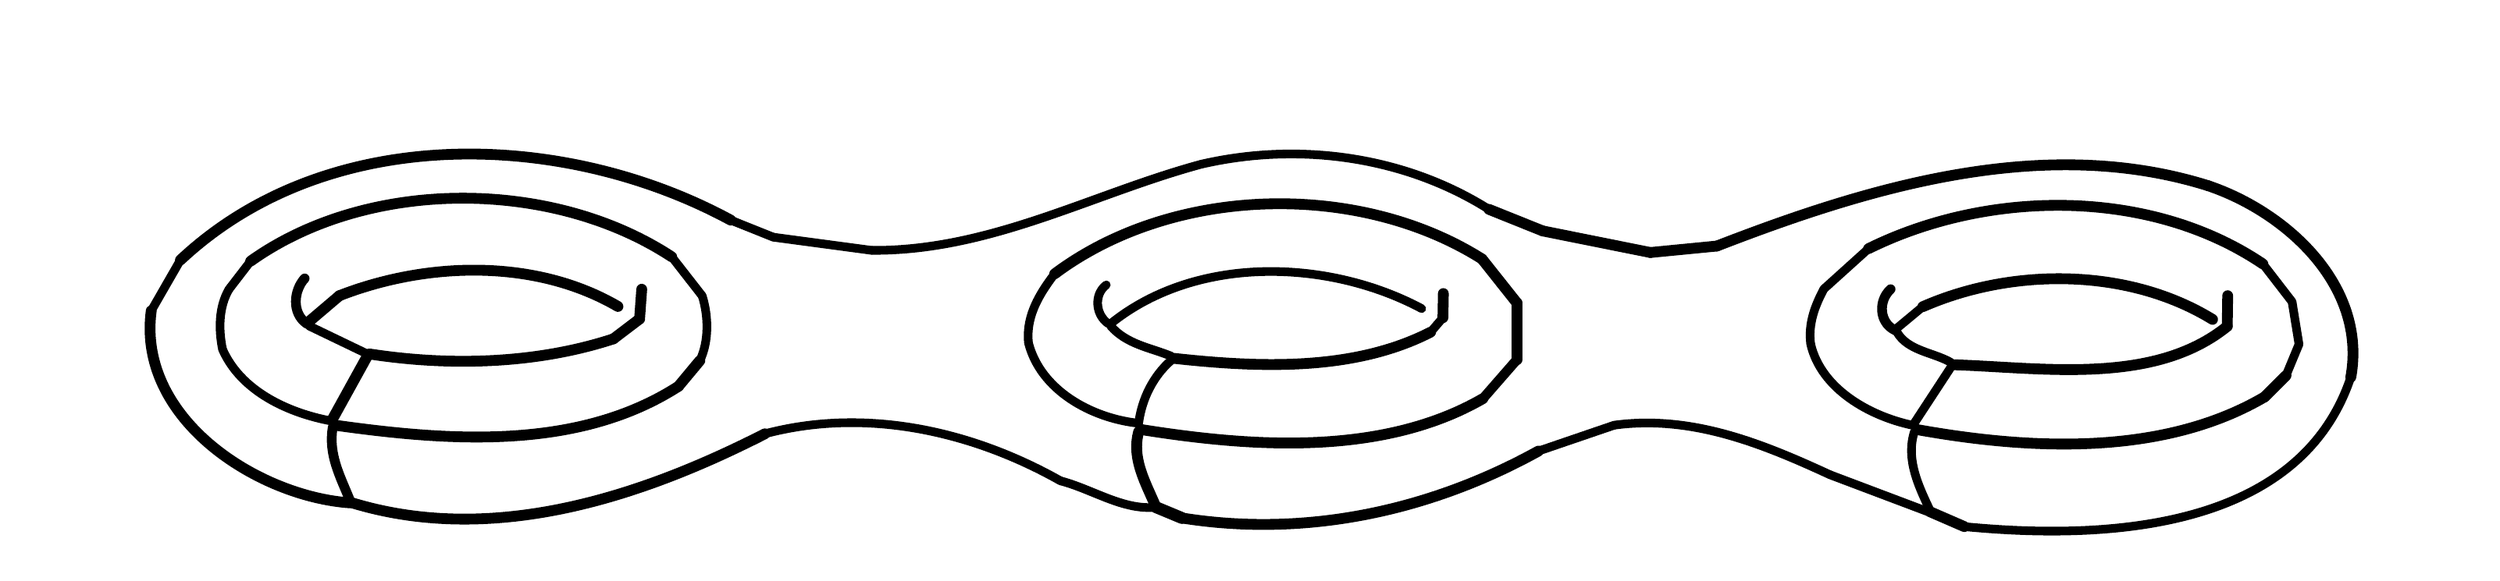
\begin{tikzpicture}[x=1pt, y=-1pt, line width=5.0pt, line cap=round, line join=round]

  %% ════ 直线段（prims2 的 strokes）════
  \draw[line width=5.0pt] (675.9,110.0) -- (692.0,130.3);
  \draw[line width=5.0pt] (692.0,130.3) -- (692.0,156.7);
  \draw[line width=4.5pt] (692.0,156.7) -- (676.3,174.7);
  \draw[line width=4.0pt] (834.1,123.9) -- (854.8,105.2);
  \draw[line width=4.0pt] (1037.3,112.3) -- (1050.8,129.8);
  \draw[line width=4.0pt] (1050.8,129.8) -- (1054.0,149.5);
  \draw[line width=4.0pt] (1054.0,149.5) -- (1048.0,164.0);
  \draw[line width=5.0pt] (1048.0,164.0) -- (1038.1,173.9);
  \draw[line width=4.0pt] (133.0,141.0) -- (160.0,154.0);
  \draw[line width=4.0pt] (876.0,186.0) -- (893.0,160.0);
  \draw[line width=5.0pt] (273.9,147.0) -- (286.0,137.8);
  \draw[line width=5.0pt] (286.0,137.8) -- (287.0,124.0);
  \draw[line width=5.0pt] (144.0,184.0) -- (160.0,155.0);
  \draw[line width=4.0pt] (652.1,143.9) -- (657.8,137.2);
  \draw[line width=5.0pt] (657.8,137.2) -- (658.0,126.0);
  \draw[line width=5.0pt] (883.0,227.0) -- (899.1,234.0);
  \draw[line width=5.0pt] (784.6,104.0) -- (753.8,107.0);
  \draw[line width=5.0pt] (753.8,107.0) -- (704.0,97.0);
  \draw[line width=5.0pt] (704.0,97.0) -- (679.1,87.0);
  \draw[line width=4.0pt] (393.4,106.0) -- (347.9,99.9);
  \draw[line width=4.0pt] (347.9,99.9) -- (328.2,92.0);
  \draw[line width=4.0pt] (73.5,110.5) -- (60.0,134.0);
  \draw[line width=5.0pt] (304.0,169.0) -- (313.9,157.1);
  \draw[line width=4.0pt] (315.0,127.1) -- (300.9,109.0);
  \draw[line width=4.0pt] (106.0,111.0) -- (96.0,124.0);
  \draw[line width=5.0pt] (147.1,127.0) -- (133.0,139.0);
  \draw[line width=5.0pt] (1021.0,127.0) -- (1020.8,141.2);
  \draw[line width=5.5pt] (525.0,225.0) -- (537.0,230.0);
  \draw[line width=4.0pt] (702.0,199.0) -- (737.1,187.0);
  \draw[line width=4.0pt] (837.0,210.0) -- (882.0,227.0);
  \draw[line width=4.0pt] (879.9,132.1) -- (868.0,142.0);

  %% ════ 曲线（prims2 的 curves —— 三段式，坐标同为 (y,x)）════
  \draw[line width=4.0pt] (516.0,186.0) .. controls (495.1,183.5) and (471.7,171.0) .. (466.0,148.9);
  \draw[line width=4.0pt] (466.0,148.9) .. controls (464.7,136.5) and (471.1,126.1) .. (478.1,116.9);
  \draw[line width=5.0pt] (478.1,116.9) .. controls (532.8,75.9) and (618.7,73.8) .. (675.9,110.0);
  \draw[line width=5.0pt] (676.3,174.7) .. controls (630.0,201.4) and (569.8,197.3) .. (518.0,189.0);
  \draw[line width=4.0pt] (532.0,157.0) .. controls (523.6,164.3) and (518.4,175.1) .. (517.0,186.0);
  \draw[line width=4.0pt] (875.0,187.0) .. controls (855.7,182.9) and (832.9,170.5) .. (828.0,149.4);
  \draw[line width=4.0pt] (828.0,149.4) .. controls (826.8,139.8) and (830.0,131.7) .. (834.1,123.9);
  \draw[line width=5.0pt] (854.8,105.2) .. controls (910.1,77.8) and (985.0,76.9) .. (1037.3,112.3);
  \draw[line width=5.0pt] (1038.1,173.9) .. controls (991.1,201.5) and (929.7,198.5) .. (877.0,189.0);
  \draw[line width=4.5pt] (152.0,222.0) .. controls (147.8,211.3) and (141.8,200.9) .. (144.0,188.0);
  \draw[line width=5.0pt] (161.0,154.0) .. controls (198.4,159.8) and (238.6,158.6) .. (273.9,147.0);
  \draw[line width=5.0pt] (533.0,156.0) .. controls (572.9,160.4) and (616.6,162.1) .. (652.1,143.9);
  \draw[line width=4.0pt] (899.1,234.0) .. controls (963.7,240.3) and (1054.2,236.3) .. (1078.0,164.7);
  \draw[line width=5.0pt] (1078.0,164.7) .. controls (1085.6,122.4) and (1048.2,88.2) .. (1011.8,76.0);
  \draw[line width=5.0pt] (1011.8,76.0) .. controls (935.5,52.1) and (854.5,76.9) .. (784.6,104.0);
  \draw[line width=4.0pt] (679.1,87.0) .. controls (640.1,62.4) and (591.3,55.6) .. (545.9,66.1);
  \draw[line width=4.0pt] (545.9,66.1) .. controls (495.3,79.8) and (448.5,106.4) .. (393.4,106.0);
  \draw[line width=5.0pt] (328.2,92.0) .. controls (250.8,50.0) and (141.4,46.7) .. (73.5,110.5);
  \draw[line width=5.0pt] (60.0,134.0) .. controls (53.3,184.1) and (109.3,220.0) .. (152.0,223.0);
  \draw[line width=4.0pt] (503.0,140.0) .. controls (496.9,135.9) and (496.2,126.4) .. (502.0,122.0);
  \draw[line width=5.0pt] (153.0,223.0) .. controls (218.4,242.9) and (286.8,220.2) .. (344.0,191.0);
  \draw[line width=4.0pt] (344.0,191.0) .. controls (391.0,178.5) and (440.3,189.9) .. (480.8,212.8);
  \draw[line width=4.0pt] (480.8,212.8) .. controls (495.5,216.6) and (509.8,226.6) .. (525.0,225.0);
  \draw[line width=4.0pt] (876.0,190.0) .. controls (871.9,202.7) and (878.0,215.3) .. (883.0,226.0);
  \draw[line width=5.0pt] (145.0,187.0) .. controls (198.3,194.5) and (257.7,198.8) .. (304.0,169.0);
  \draw[line width=4.0pt] (313.9,157.1) .. controls (318.2,148.1) and (317.9,136.5) .. (315.0,127.1);
  \draw[line width=5.0pt] (300.9,109.0) .. controls (245.6,72.6) and (160.2,72.3) .. (106.0,111.0);
  \draw[line width=4.0pt] (96.0,124.0) .. controls (91.2,132.1) and (91.1,142.7) .. (93.0,151.9);
  \draw[line width=4.0pt] (93.0,151.9) .. controls (101.6,171.4) and (123.5,181.3) .. (143.0,185.0);
  \draw[line width=5.0pt] (276.0,132.0) .. controls (237.8,109.7) and (187.6,111.2) .. (147.1,127.0);
  \draw[line width=4.0pt] (893.0,158.0) .. controls (885.1,153.3) and (873.1,152.7) .. (868.0,144.0);
  \draw[line width=5.0pt] (1020.8,141.2) .. controls (986.8,168.8) and (935.2,160.3) .. (894.0,159.0);
  \draw[line width=4.0pt] (504.0,141.0) .. controls (511.4,149.6) and (522.5,151.1) .. (532.0,155.0);
  \draw[line width=4.5pt] (867.0,143.0) .. controls (859.6,139.4) and (859.2,129.3) .. (865.0,124.0);
  \draw[line width=5.0pt] (525.0,225.0) .. controls (520.5,214.1) and (513.5,202.6) .. (517.0,190.0);
  \draw[line width=5.0pt] (537.0,230.0) .. controls (595.0,239.3) and (652.5,226.4) .. (702.0,199.0);
  \draw[line width=4.0pt] (737.1,187.0) .. controls (773.1,182.1) and (806.0,195.7) .. (837.0,210.0);
  \draw[line width=4.5pt] (131.0,119.0) .. controls (126.0,124.5) and (124.8,135.0) .. (132.0,140.0);
  \draw[line width=5.0pt] (1014.0,138.0) .. controls (975.0,114.0) and (921.3,113.9) .. (879.9,132.1);
  \draw[line width=4.0pt] (504.0,140.0) .. controls (543.7,107.9) and (605.0,110.0) .. (648.0,133.0);

  %% ════ 标签（probe 直接给的 \node 行）════
  %% ⚠ 全部补了 fill=white：文字在最上层，否则与曲线交叉干扰

  % 钉死画布：否则超出的图元/控制点会把页面撑大，1:1 回比就失准
  \pgfresetboundingbox
  \path[use as bounding box] (0,0) rectangle (1137,249);
\end{tikzpicture}
\end{document}

% ⚠ 待核清单（probe 拿不准，人眼过一遍）：
%   · 未识别/跳过：⑤ 跳过/未识别的字形
